%%
%% This is file `sample-sigconf.tex',
%% generated with the docstrip utility.
%%
%% The original source files were:
%%
%% samples.dtx  (with options: `sigconf')
%% 
%% IMPORTANT NOTICE:
%% 
%% For the copyright see the source file.
%% 
%% Any modified versions of this file must be renamed
%% with new filenames distinct from sample-sigconf.tex.
%% 
%% For distribution of the original source see the terms
%% for copying and modification in the file samples.dtx.
%% 
%% This generated file may be distributed as long as the
%% original source files, as listed above, are part of the
%% same distribution. (The sources need not necessarily be
%% in the same archive or directory.)
%%
%% The first command in your LaTeX source must be the \documentclass command.
\documentclass[sigplan,review]{acmart}

\usepackage{code}
\usepackage{graphicx}

%%
%% \BibTeX command to typeset BibTeX logo in the docs
\AtBeginDocument{%
  \providecommand\BibTeX{{%
    \normalfont B\kern-0.5em{\scshape i\kern-0.25em b}\kern-0.8em\TeX}}}

%% Rights management information.  This information is sent to you
%% when you complete the rights form.  These commands have SAMPLE
%% values in them; it is your responsibility as an author to replace
%% the commands and values with those provided to you when you
%% complete the rights form.
\setcopyright{acmcopyright}
\copyrightyear{2021}
\acmYear{2021}
\acmDOI{10.1145/1122445.1122456}

%% These commands are for a PROCEEDINGS abstract or paper.
\acmConference[Woodstock '18]{Woodstock '18: ACM Symposium on Neural
  Gaze Detection}{June 03--05, 2018}{Woodstock, NY}
\acmBooktitle{Woodstock '18: ACM Symposium on Neural Gaze Detection,
  June 03--05, 2018, Woodstock, NY}
\acmPrice{15.00}
\acmISBN{978-1-4503-XXXX-X/18/06}


%%
%% Submission ID.
%% Use this when submitting an article to a sponsored event. You'll
%% receive a unique submission ID from the organizers
%% of the event, and this ID should be used as the parameter to this command.
%%\acmSubmissionID{123-A56-BU3}

%%
%% The majority of ACM publications use numbered citations and
%% references.  The command \citestyle{authoryear} switches to the
%% "author year" style.
%%
%% If you are preparing content for an event
%% sponsored by ACM SIGGRAPH, you must use the "author year" style of
%% citations and references.
%% Uncommenting
%% the next command will enable that style.
%%\citestyle{acmauthoryear}

%%
%% end of the preamble, start of the body of the document source.
\begin{document}

%%
%% The "title" command has an optional parameter,
%% allowing the author to define a "short title" to be used in page headers.
\title{Let a Thousand Flowers Bloom: on the Uses of Diversity in
  Software Testing}

%%
%% The "author" command and its associated commands are used to define
%% the authors and their affiliations.
%% Of note is the shared affiliation of the first two authors, and the
%% "authornote" and "authornotemark" commands
%% used to denote shared contribution to the research.
\author{Alex Groce}
\affiliation{\institution{Northern Arizona University}\country{United States}}


%%
%% By default, the full list of authors will be used in the page
%% headers. Often, this list is too long, and will overlap
%% other information printed in the page headers. This command allows
%% the author to define a more concise list
%% of authors' names for this purpose.
\renewcommand{\shortauthors}{Alex Groce}

%%
%% The abstract is a short summary of the work to be presented in the
%% article.
\begin{abstract}
Software testing is \emph{hard}; like many real-world problems, it
offers no optimal solution, but requires dexterity, and the
opportunistic combination of many partial solutions.  Exploration and
experiment, even by practitioners, are important in real-world
critical testing efforts.  An important set of research results in the
field endorse and codify the value of \emph{diversity} in the field.
However, our current approaches to evaluating research results
arguably cut against this fundamental reality: while effective testing
may need true diversity, combining many partial answers, the iron
logic of the research results section often imposes a
\emph{totalizing} vision where authors must at least pretend to
present a monolithic Solution with a capital ``S.''
\end{abstract}

\begin{CCSXML}
<ccs2012>
<concept>
<concept_id>10011007.10010940.10010992.10010998.10011001</concept_id>
<concept_desc>Software and its engineering~Dynamic analysis</concept_desc>
<concept_significance>500</concept_significance>
</concept>
<concept>
<concept_id>10011007.10011074.10011099.10011102.10011103</concept_id>
<concept_desc>Software and its engineering~Software testing and debugging</concept_desc>
<concept_significance>500</concept_significance>
</concept>
</ccs2012>
\end{CCSXML}

\ccsdesc[500]{Software and its engineering~Dynamic analysis}
\ccsdesc[500]{Software and its engineering~Software testing and debugging}

\keywords{test diversity, swarm testing, ensemble methods,
  test length}


\maketitle

\section{Introduction}

\section{Diversity in Practice}

\subsection{Swarm Techniques}

\begin{figure}
  \centering
  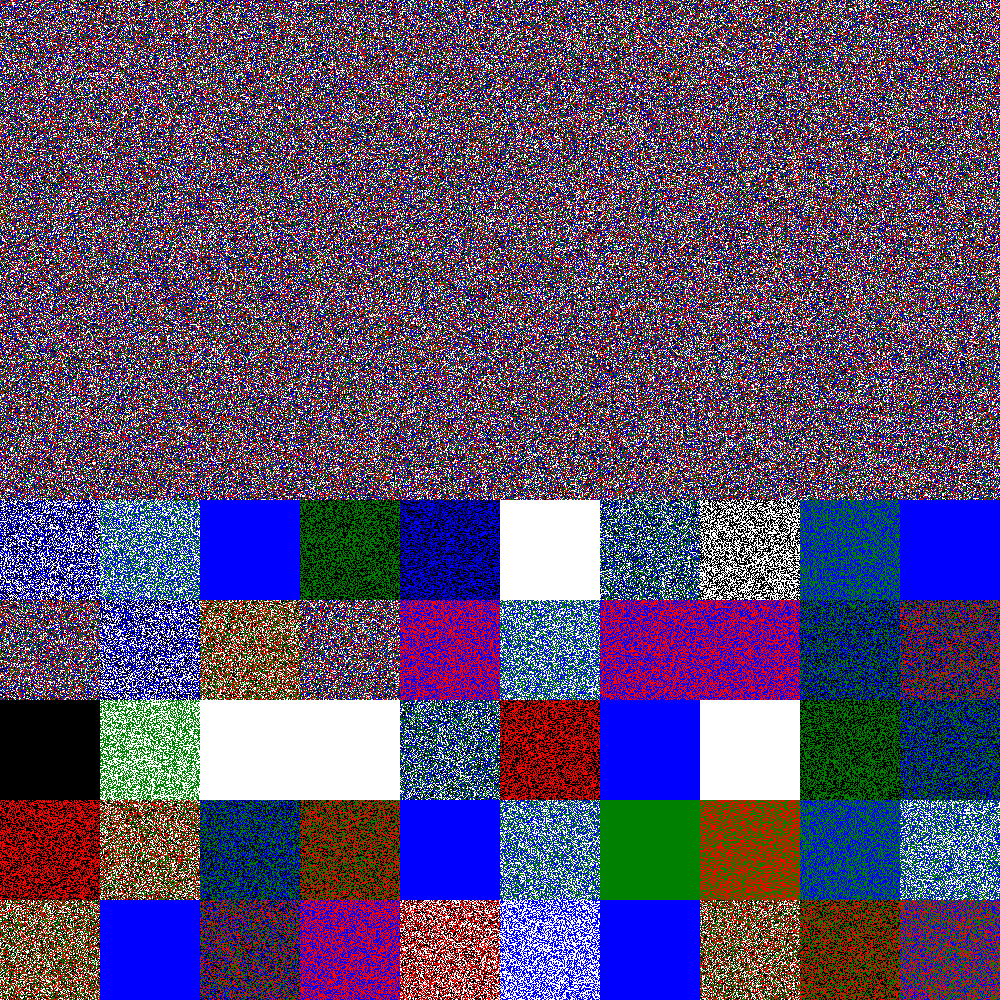
\includegraphics[width=\columnwidth]{swarm.png}
  \caption{Kitchen-sink (top) vs. Swarm (bottom)}
  \label{fig:swarmcol}
\end{figure}


\subsection{Ensemble Methods}



\subsection{Test Length}

\subsection{Tools}

\section{The Totalizing Nature of the Experimental Results Section}



Swarm testing \cite{ISSTA12} is pretty cool.

\bibliographystyle{plain}
\bibliography{bibliography}



\end{document}